\section{Введение в тематическое моделирование}
\begin{frame}[t]{Задача тематического моделирования}
\textbf{Дано:}
\begin{itemize}
    \item $D$ --- коллекция текстовых документов
    \item $W$ --- множество уникальных термов коллекции
    \item $n_{dw}$ --- число вхождений слова $w$ в <<мешок слов>> документа $d$
\end{itemize}

\medskip
\textbf{Найти:}
множество тем $T$ и два семейства распределений:
\smallskip
\begin{itemize}
    \item $p(w \cond t)$ --- распределения термов в темах
    \item $p(t \cond d)$ --- распределения тем в документах
\end{itemize}

\[
p(w \cond d) = \sum_{t \in T} p(w \cond t)p(t \cond d) = \sum_{t \in T} \phi_{wt}\theta_{td}
\]

\smallskip
\textbf{Критерий:} максимум правдоподобия с регуляризаторами $\tau_i R_i$:
\[
    \sum_{d \in D} \sum_{w \in d} n_{dw} \mathrm{ln} \sum_{t \in T} \phi_{wt} \theta_{td} + R(\Phi, \Theta) \rightarrow \underset{\Phi, \Theta}{\mathrm{max}}, \quad R(\Phi, \Theta) = \sum_{i} \tau_i R_i(\Phi, \Theta)
\]
\[
\phi_{wt} \ge 0; \quad \sum_{w \in W} \phi_{wt} = 1; \quad \theta_{td} \ge 0; \quad \sum_{d \in D} \theta_{td} = 1.
\]
\bigskip

\footnotetext{
Воронцов К. В. Аддитивная регуляризация тематических моделей коллекций текстовых документов // Доклады РАН. 2014.}
\end{frame}

\begin{frame}{Гиперпараметры тематических моделей}
\begin{itemize}
    \item У большинства тематических моделей: число тем $T$
    \item У LDA: $\alpha$, $\eta$
    \item В ARTM: коэффициенты регуляризации
\end{itemize}
\end{frame}

\begin{frame}[t]{Проблемы практического применения тематических моделей}

С какими проблемами сталкиваются пользователи тематических моделей?
\begin{enumerate}
    \item Неинтерпретируемые или плохо интерпретируемые темы
    \item Вводящие в заблуждение темы
    \item Дублирующие темы
    \item Мусорные темы
    \item Неустойчивость
\end{enumerate}
В теории настройка гиперпараметров может устранить проблемы 3, 4, 5. Если существовали бы процедуры измерения интерпретируемости и регламент валидации, то настройка гиперпараметров могла бы помочь и с проблемами 1 и 2.
\end{frame}
\note{
В теории именно настройка гиперпараметров отличает плохую модель от хорошей.

Что такое плохая тематическая модель?
Ну, я выделю ряд проблем важных на практике. Пойду снизу вверх.

Неустойчивость --- не позволяет говорить о какой-то определённой модели. Связана как минимум с числом тем. Разреживание позволяет уменьшить число валидных локальных максимумов.

Мусорные темы --- совсем избавиться от них нельзя, но в теории их можно изолировать.

Дублирующие темы --- плохо потому что не даёт исследователю информации. Стандартный регуляризатор декорреляции хорошо с этим справляется.

Вводящие в заблуждение темы --- нужны инструменты визуализации.

Неинтерпретируемые --- нужны критерии качества.
}

\begin{frame}{Настройка гиперпараметров тематических моделей}
Проблема: никто не умеет подбирать гиперпараметры. В статье\footnote{Chen T. H., Thomas S. W., Hassan A. E. A survey on the use of topic models when mining software repositories //Empirical Software Engineering. – 2016.} сделали обзор 167 статей: 45\% работ не указывает использованное значение $T$ вовсе, 33\% приводит его без разъяснений о том, как оно было выбрано, 9\% используют перебор различных значений.

\bigskip

Проблема: непонятно, как измерять интерпретируемость. Когерентность плохо взаимодействует со стоп-словами. Попытки определить плохие темы через расстояние до известных <<мусорных>> тем или через низкие значения когерентности дают лишь срез проблематичных тем и имеют ограниченную область применимости.

\end{frame}


\begin{frame}[t]{Цель и задачи диссертационного исследования}
\textbf{Цель:} разработка технологии построения интерпретируемых  тематических моделей, применимых для решения широкого класса задач тематического моделирования.

\bigskip
\textbf{Задачи:}
\begin{enumerate}
    \smallskip\item Автоматические критерии интерпретируемости: реализация, эмпирическое исследование, улучшение; новый критерий внутритекстовой когерентности.

    \smallskip\item Разработка методологии и средств автоматизации проведения экспериментов по подбору стратегии регуляризации и выбору гиперпараметров тематической модели.

    \smallskip\item Проектирование архитектуры библиотеки TopicNet; пользовательские регуляризаторы и метрики качества в TopicNet.

    \smallskip\item Поиск универсального <<рецепта>> построения тематических моделей, превосходящих LDA по ряду критериев качества.

    \smallskip\item Решение прикладных задач с использованием разработанной библиотеки TopicNet.

\end{enumerate}
\end{frame}

% \begin{frame}[t]{Доступность тематических моделей}

% Таким образом, принятые методологии перекладывают ответственность за подбор гиперпараметров на исследователя; при этом процедура подбора остаётся нерегламентированной, что создаёт высокий барьер входа для неспециалистов. 

% В~обзорной монографии \cite{fntir2017applications} подчёркивается важность снижения порога входа и более жёсткой регламентации процесса моделирования: <<первоочередная исследовательская задача в тематическом моделировании... сделать его более доступным>>.

% \end{frame}

\section{Методология построения ТМ в библиотеке TopicNet}



\begin{frame}{Верхние токены}


\begin{enumerate}
    \item Для каждой темы выбирается какой-то небольшой набор характеризующих её токенов (как правило, это 10 верхних токенов).
    \item{Этот набор анализируется одним из двух способов:
    \begin{itemize}
        \item качество тем оценивается экспертом визуально по этим токенам;
        \item качество тем оценивается путём автоматического вычисления определённых статистик, в частности, парной сочетаемости верхних токенов в текстовой коллекции.
    \end{itemize}
    }
    % \fixme{тут бы картинку сделать?}
\end{enumerate}

\end{frame}

\begin{frame}{Верхние токены}

Ориентирующийся на когерентность исследователь неявно рассуждает таким образом:
\begin{enumerate}
    \item Верхние токены темы имеют высокую когерентность;
    \item Верхние токены темы встречаются в документах согласованным образом;
    \item Все токены темы встречаются в документах согласованным образом;
    \item Тема является хорошей.
\end{enumerate}

\end{frame}
\begin{frame}{Доля текста, покрытая верхними словами}

\begin{figure}
    %\begin{tabular}{p{7.5cm}p{3.5cm}}
        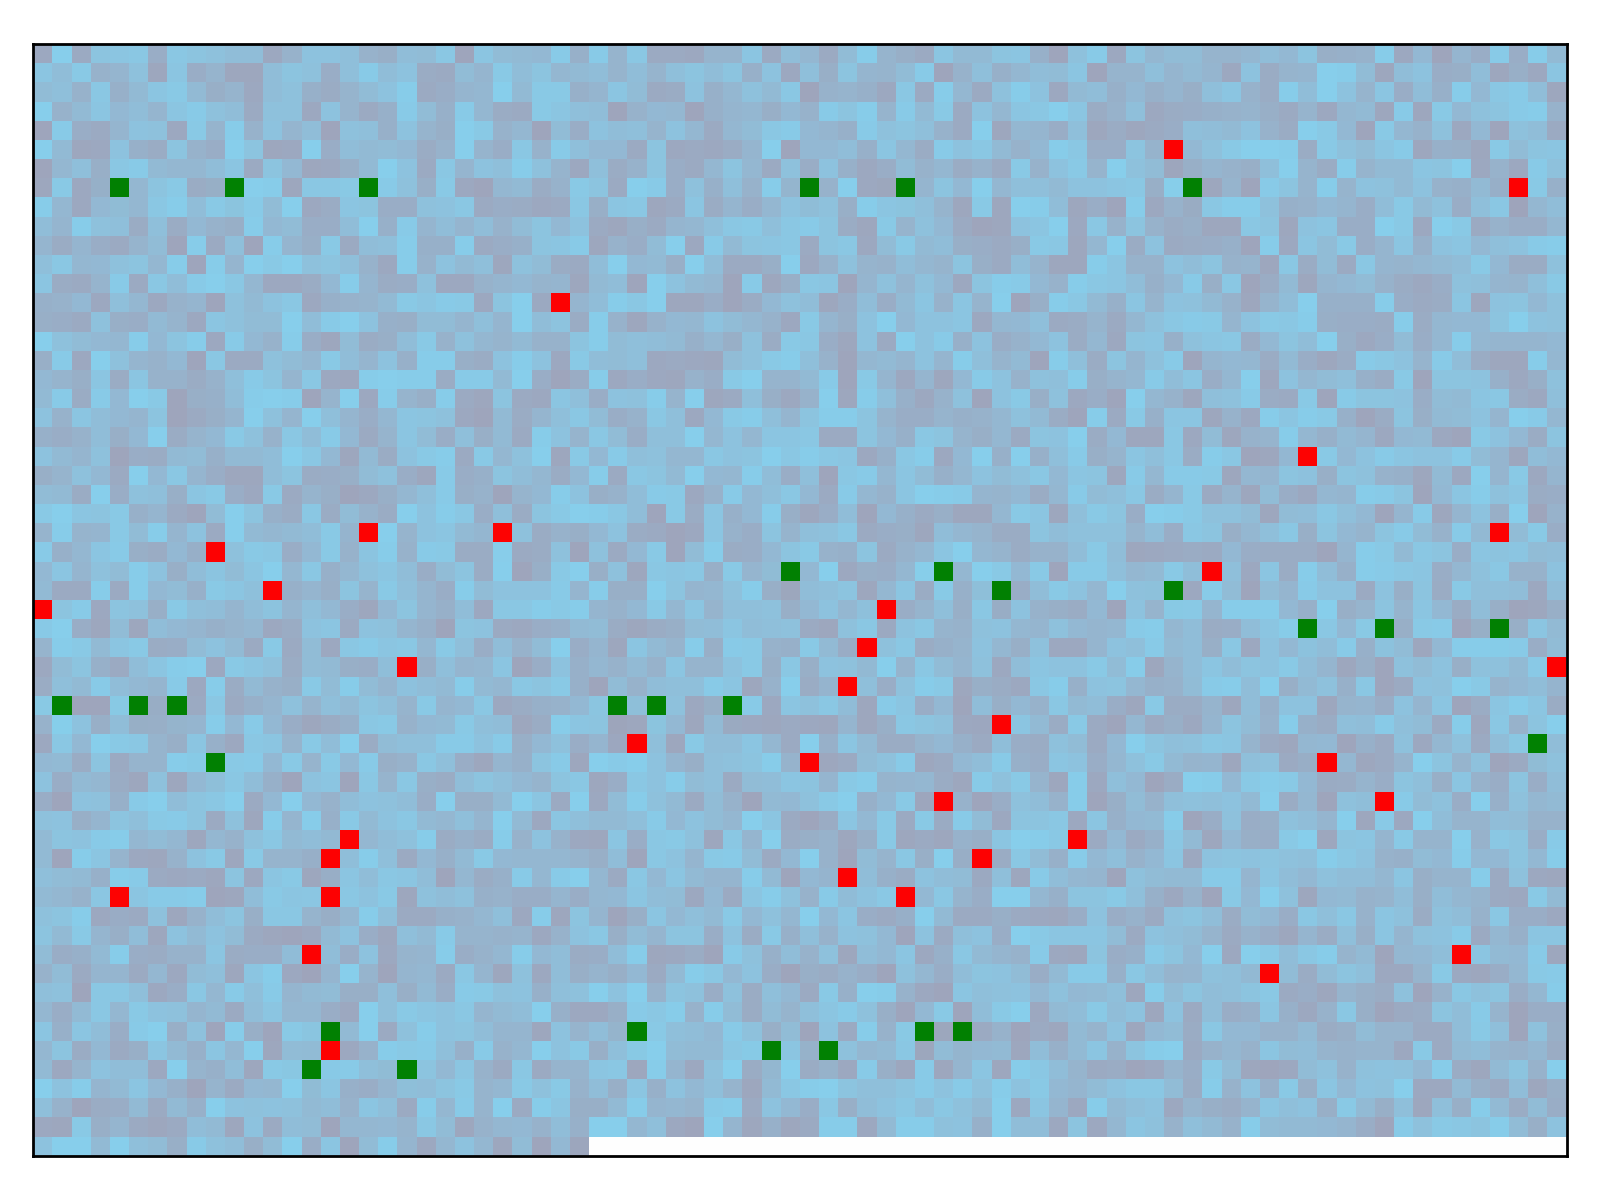
\includegraphics[width=0.75\textwidth]{doc11358_topic0.png} %&
        % 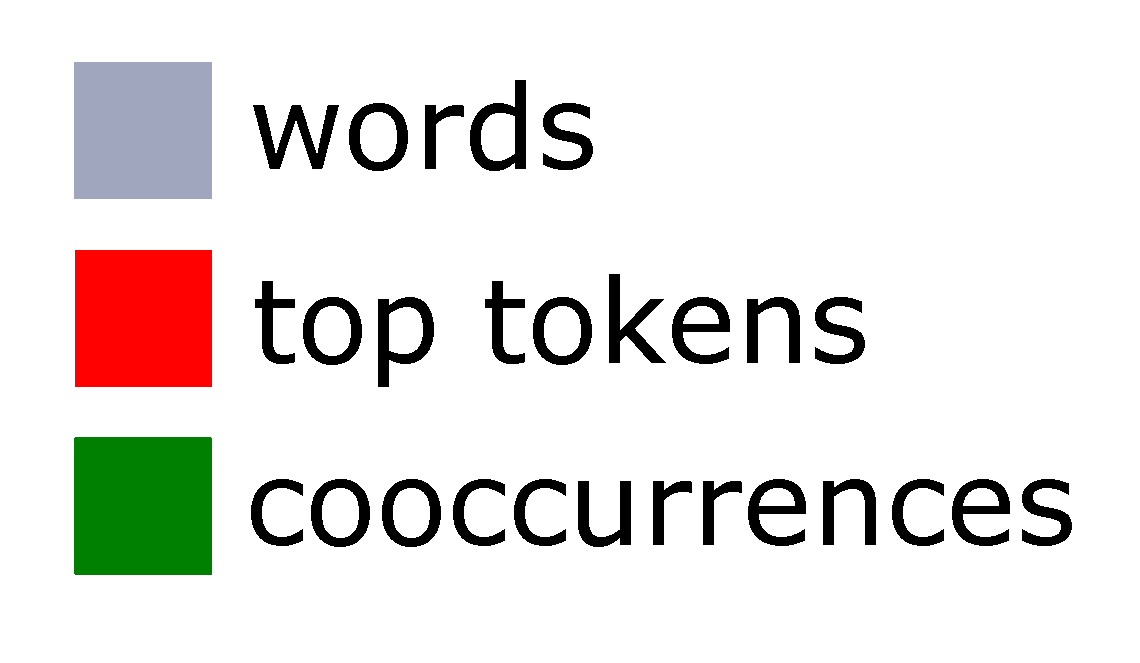
\includegraphics[width=0.25\textwidth]{legend.eps} \\
    %\end{tabular}
\end{figure}
\vspace{-7pt}
Словопозиции обозначены серо-синим цветом, словопозиции верхних слов показаны красным цветом, зелёным цветом показаны словопозиции, имеющие ненулевой вклад в расчёт когерентности (т.е. попадающие в скользящее окно вместе с другим верхним словом).
\end{frame}

\begin{frame}{Доля текста, покрытая верхними словами}

\begin{table}[ht]
\begin{tabular}{|l|l|l|} \hline
         & ПостНаука & Википедия \\ \hline
Минимум  & 0.0159\%  & 0.0065\%  \\ \hline
Медиана  & 0.0483\%  & 0.0293\%  \\ \hline
Среднее  & 0.0619\%  & 0.0356\%  \\ \hline
Максимум & 0.2764\%  & 0.1149\%  \\ \hline
Суммарно & 1.2027\%  & 1.6585\%  \\ \hline
\end{tabular}
\end{table}
      Доля коллекции, имеющая ненулевой вклад в счётчики парных сочетаемостей 10 верхних слов. Статистики посчитаны по каждой теме отдельно; строка <<суммарно>> показывает представительность объединённого множества верхних слов всех тем.
\end{frame}


\begin{frame}{Внутритекстовая когерентность}

\begin{figure}
    \centering
    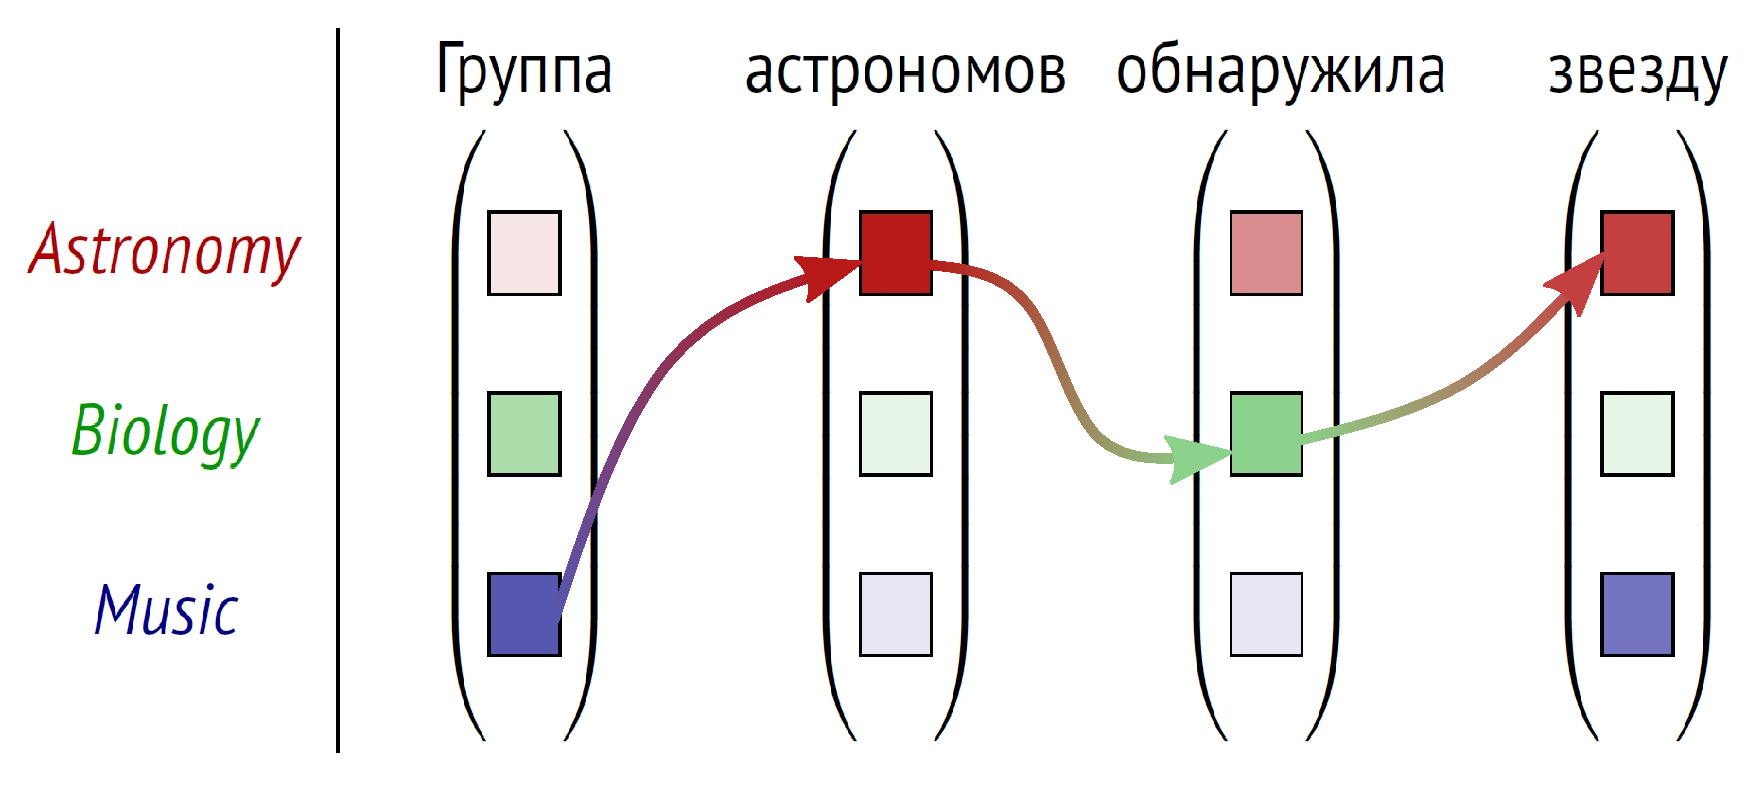
\includegraphics[width=0.8\textwidth, height=0.3\textheight]{astronomers_focon.eps} % .eps image is wrong scaled
\end{figure}

Идея: выделить все соседние слова текста и анализировать их распределение $\phi_{wt}$.\\
\medskip
(вместо того, чтобы выделять небольшое множество слов при помощи $\phi_{wt}$ и затем анализировать, как эти слова встречаются в тексте)

\end{frame}

\begin{frame}{Внутритекстовая когерентность}

\begin{figure}
\begin{tabular}{cc}
    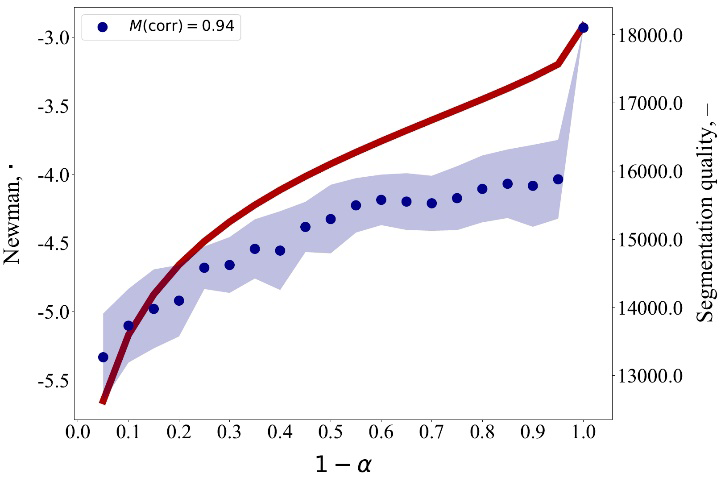
\includegraphics[width=70mm]{images/segm_mimno.png}
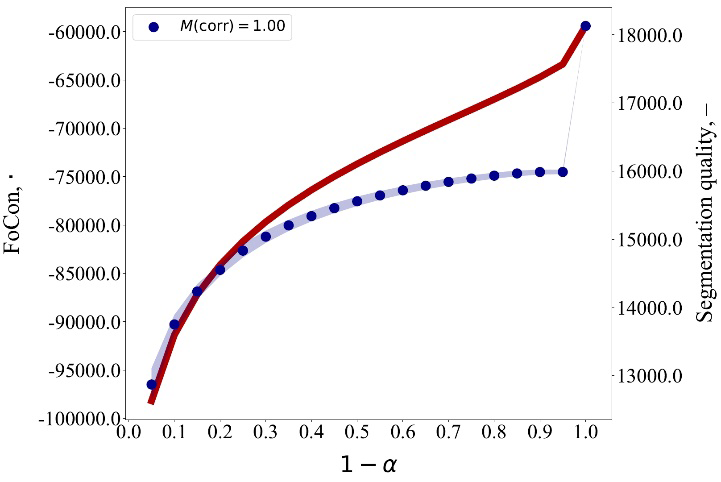
\includegraphics[width=70mm]{images/segm_focon.png} \\
\end{tabular}
\end{figure}

Сравнение различных мер когерентности и качества сегментации, нарисованное как функция от степени деградации тематической модели $\alpha$.

\end{frame}

\begin{frame}{Относительные коэффициенты регуляризации}
Общие формулы:
\[
\theta_{td} = \norm_{t \in T} \Bigg(
    n_{td} + \sum_{i=1}^k \lambda_i \Big[
        \frac{n}{\sum_{d\in D} r_{id}}
        \Big]
    \theta_{td} \frac{\partial R_i}{\partial \theta_{td}}
\Bigg)
\]


\[
\phi_{wt} = \norm_{w \in W}\Bigg(
    n_{wt} + \sum_{i=1}^k \lambda_i \Big[
        \frac{n}{\sum_{t\in T} r_{it}}
        \Big]
    \phi_{wt} \frac{\partial R_i}{\partial \phi_{wt}}
\Bigg)
\]

\small
\begin{itemize}
    \item { $r_{id} = \sum_{t\in T} \Big | \theta_{td} \frac{\partial R_i}{\partial \theta_{td}} \Big | $ --- воздействие регуляризатора на документ}

    \item{$r_{it} = \sum_{w\in W} \Big| \phi_{wt} \frac{\partial R_i}{\partial \phi_{wt}} \Big| $ --- воздействие регуляризатора на тему}
	\item { $\lambda_i$ - относительный коэффициент регуляризации, показывающий, \emph{во сколько раз} соответствующий регуляризатор влияет на оценку матриц больше, чем коллекция}
\end{itemize}

Случай $\phi_{wt}$ реализован в BigARTM, случай $\theta_{td}$~--- нет (поскольку $r_{id}$ недоступен при параллельной реализации).

\end{frame}

\begin{frame}{Сглаживание и разреживание}
Для регуляризаторов сглаживания/разреживания ($\Phi$ или $\Theta$) формула существенно упрощается!

\begin{table}[]
\begin{tabular}{l|c|c|}
         & \multicolumn{2}{c}{Управляющий параметр}                                                                                                      \\ \hline
         & $\tau$                                          & $\lambda$                                                                                   \\ \hline 
         &    &          \\[-5pt]
$\Phi$   & $\phi_{wt} = \norm_{w \in W}\Bigg(n_{wt} + \tau\Bigg)$    & $\phi_{wt} = \norm_{w \in W}\Bigg(n_{wt} + \lambda {\color{red}\frac{n}{|W||T|}}\Bigg)$    \\[15pt] \hline
         &    &          \\[-5pt]
$\Theta$ & $\theta_{td} = \norm_{t \in T} \Bigg(n_{td} + \tau\Bigg)$ & $\theta_{td} = \norm_{t \in T} \Bigg(n_{td} + \lambda {\color{red}\frac{n}{|D| |T|}}\Bigg)$ \\[15pt]  \hline
\end{tabular}
\end{table}
Вывод: сглаживание/разреживание с абсолютным коэффициентом и относительным эквивалентно 

\smallskip
(в частности, можно вычислить абсолютный коэффициент сглаживания $\Theta$, эквивалентный заданному относительному).

\end{frame}

\begin{frame}{Репараметризация сглаживания/разреживания}
	
\begin{equation}
\tau = \frac{n}{|D| \cdot |T|} \frac{\lambda}{(1-\lambda)}
\end{equation}

\begin{equation}
\tau = \frac{n}{|W|\cdot|T|} \frac{\lambda}{(1-\lambda)}  
\end{equation}

Интерпретация: берём $\lambda$ частей априорного распределения
\[
\frac{1}{|T|}\text{ или }\frac{1}{|W|}
\]
и $(1-\lambda)$ частей от оценки максимума правдоподобия 
\[
\frac{n_{td}}{n_d}\text{ или }\frac{n_{wt}}{n_t}
\]

\end{frame}

\begin{frame}{относительные веса модальностей}
Формула общего правдоподобия для мультимодального случая:

\[
L(\Phi^m, \Theta) = \sum_m \tau_m \sum_{d\in D} \sum_{w \in W^m} n_{dw} \ln p(w \cond d) \rightarrow \max, 
\]

где коэффициенты $\tau_m$ показывают \textit{вес} модальности $m$. Проинтерпретируем это выражение как введение $M-1$ дополнительного регуляризатора $\Theta$ с коэффициентами $\tau_m$. Тогда $n(\sum_{d\in D} r_{id})^{-1}$ тоже выражается через константы, известные ещё на этапе построения коллекции:

\[
\tau_m = \lambda_m \frac{n}{\sum_d n_d^{(m)}} \iff
\lambda_m = \tau_m \frac{\sum_d n_d^{(m)}}{n}
\]

\end{frame}


\begin{frame}{Второстепенность матрицы Тета}

Матрица $\Theta$ является менее важной, чем $\Phi$. На практике хочется её не хранить, а восстанавливать <<на лету>>.

\begin{itemize}
\item Оценка интерпретируемости: обычно используется только матрица $\Phi$.

\item Динамическое расширение коллекции документов: сильно увеличивается $|D|$, $|W|$ растёт медленнее.

\item Пакетный EM-алгоритм: разные документы обрабатываются разными потоками. Используется $\theta_d$, а не матрица $\Theta$ целиком.
\end{itemize}

\end{frame}

\begin{frame}[t]{$\Theta$ может скомпенсировать <<плохую>> $\Phi$}

Коллекция из 3 документов: 
\begin{figure}[t]
\begin{minipage}[t]{0.4\textwidth}
	\medskip
\begin{itemize}
    \item \texttt{herbs and spices}
    \item \texttt{spices and medicine}
    \item \texttt{herbs and medicine}
\end{itemize}
	\end{minipage}
	% $\qquad\quad$
	\begin{minipage}[t]{0.4\textwidth}
\begin{center}
\begin{tabular}{l|llll}
$n_{dw}$   & and & herbs & spices & medicine \\ \hline
doc1       & 1   & 1     & 1      & 0        \\
doc2       & 1   & 0     & 1      & 1        \\
doc3       & 1   & 1     & 0      & 1      
\end{tabular}
\end{center}

\end{minipage}
\end{figure}

Есть много локальных оптимумов с зашумлённой $\Phi$, недостатки которой  <<спрятаны>>  при помощи нулей в матрице $\Theta$:
\small
\begin{minipage}[t]{0.4\textwidth}
\[
\Phi =
\begin{pmatrix}
    0.044 & 0.956 & 0 & 0 \\
    0.488 & 0 &  0 & 0.512 \\
    0.488 & 0 & 0.512 & 0   \\
    0.281 & 0 & 0.279 & 0.44 \\
\end{pmatrix},
\]
	\end{minipage}
	$\qquad\quad$
	\begin{minipage}[t]{0.4\textwidth}
\[
\Theta =
\begin{pmatrix}
    0.349 & 0 & 0.651 & 0 \\
    0 & 0.008 & 0.244 & 0.748 \\
    0.348 & 0.652 & 0 & 0 \\
\end{pmatrix}.
\]
\end{minipage}
\bigskip
\[
\Phi \cdot \Theta \approx \frac{1}{3} n_{dw}
\]
\normalsize
\end{frame}

\begin{frame}[t]{EM-алгоритм при $\Theta=f(\Phi)$ [Ирхин, 2020]}
По этим соображениям явно введём зависимость $\Theta = f(\Phi)$. Получается другая оптимизационная задача:

\begin{equation} \label{eq:tEM}
L(\Phi, f(\Phi) ) + R(\Phi, f(\Phi) ) \to \max_{\Phi},
\end{equation}
\small
\begin{Theorem}
    Пусть функция $R(\Phi,\Theta)$ непрерывно дифференцируема, а $\Theta$ находится в функциональной зависимости от $\Phi$ согласно формуле    $\theta_{td}(\Phi)
    = \norm_{t\in T} \biggl( \sum_{w\in W} n_{dw} p_{tdw} \biggr)$.
    Тогда точка $\Phi$ локального максимума 
    удовлетворяет системе уравнений со вспомогательными переменными $h_w,\ \theta_{td},\ p_{tdw},\ c_{td},\ \gamma_{dw}$:
\[
    \phi_{wt} = \norm_{w\in W}
        \Biggl(\,
        \sum_{d\in D} n_{dw} p_{tdw} 
        + \sum_{d\in D} n_{dw} n_d^{-1} \phi_{wt}h_w (c_{td}-h_w\gamma_{dw}) 
        + 
            \phi_{wt} \frac{\partial{R}}{\partial{\phi_{wt}}}
        \Biggr)
\]
\end{Theorem}
\normalsize
\end{frame}

\begin{frame}[t]{Псевдорегуляризатор быстрой векторизации}
\begin{minipage}[t]{0.99\textwidth}

\begin{align*}
    \phi_{wt} = \norm_{w\in W}
        \Biggl(\,&
        \sum_{d\in D} n_{dw} p_{tdw} \\
        + &\underbrace{\sum_{d\in D} n_{dw} n_d^{-1} \phi_{wt}h_w (c_{td}-h_w\gamma_{dw})}_{
            \let\scriptstyle\textstyle
            \substack{\textup{очень похоже на регуляризатор}}
        } \\ 
        + &\underbrace{
            \phi_{wt} \frac{\partial{R}}{\partial{\phi_{wt}}}
          }_{
          \let\scriptstyle\textstyle
            \substack{\textup{регуляризатор}}
        }
        \Biggr)
\end{align*}
\end{minipage}

Вывод: обучение можно <<сэмулировать>> внутри BigARTM, введя фиктивный псевдорегуляризатор и положив \texttt{num\_document\_passes\ =\ 1}.

\end{frame}


\begin{frame}{Влияние на тематическую модель}

\begin{figure}
\setlength\tabcolsep{0pt} % default value: 6pt
\begin{tabular}{cc}
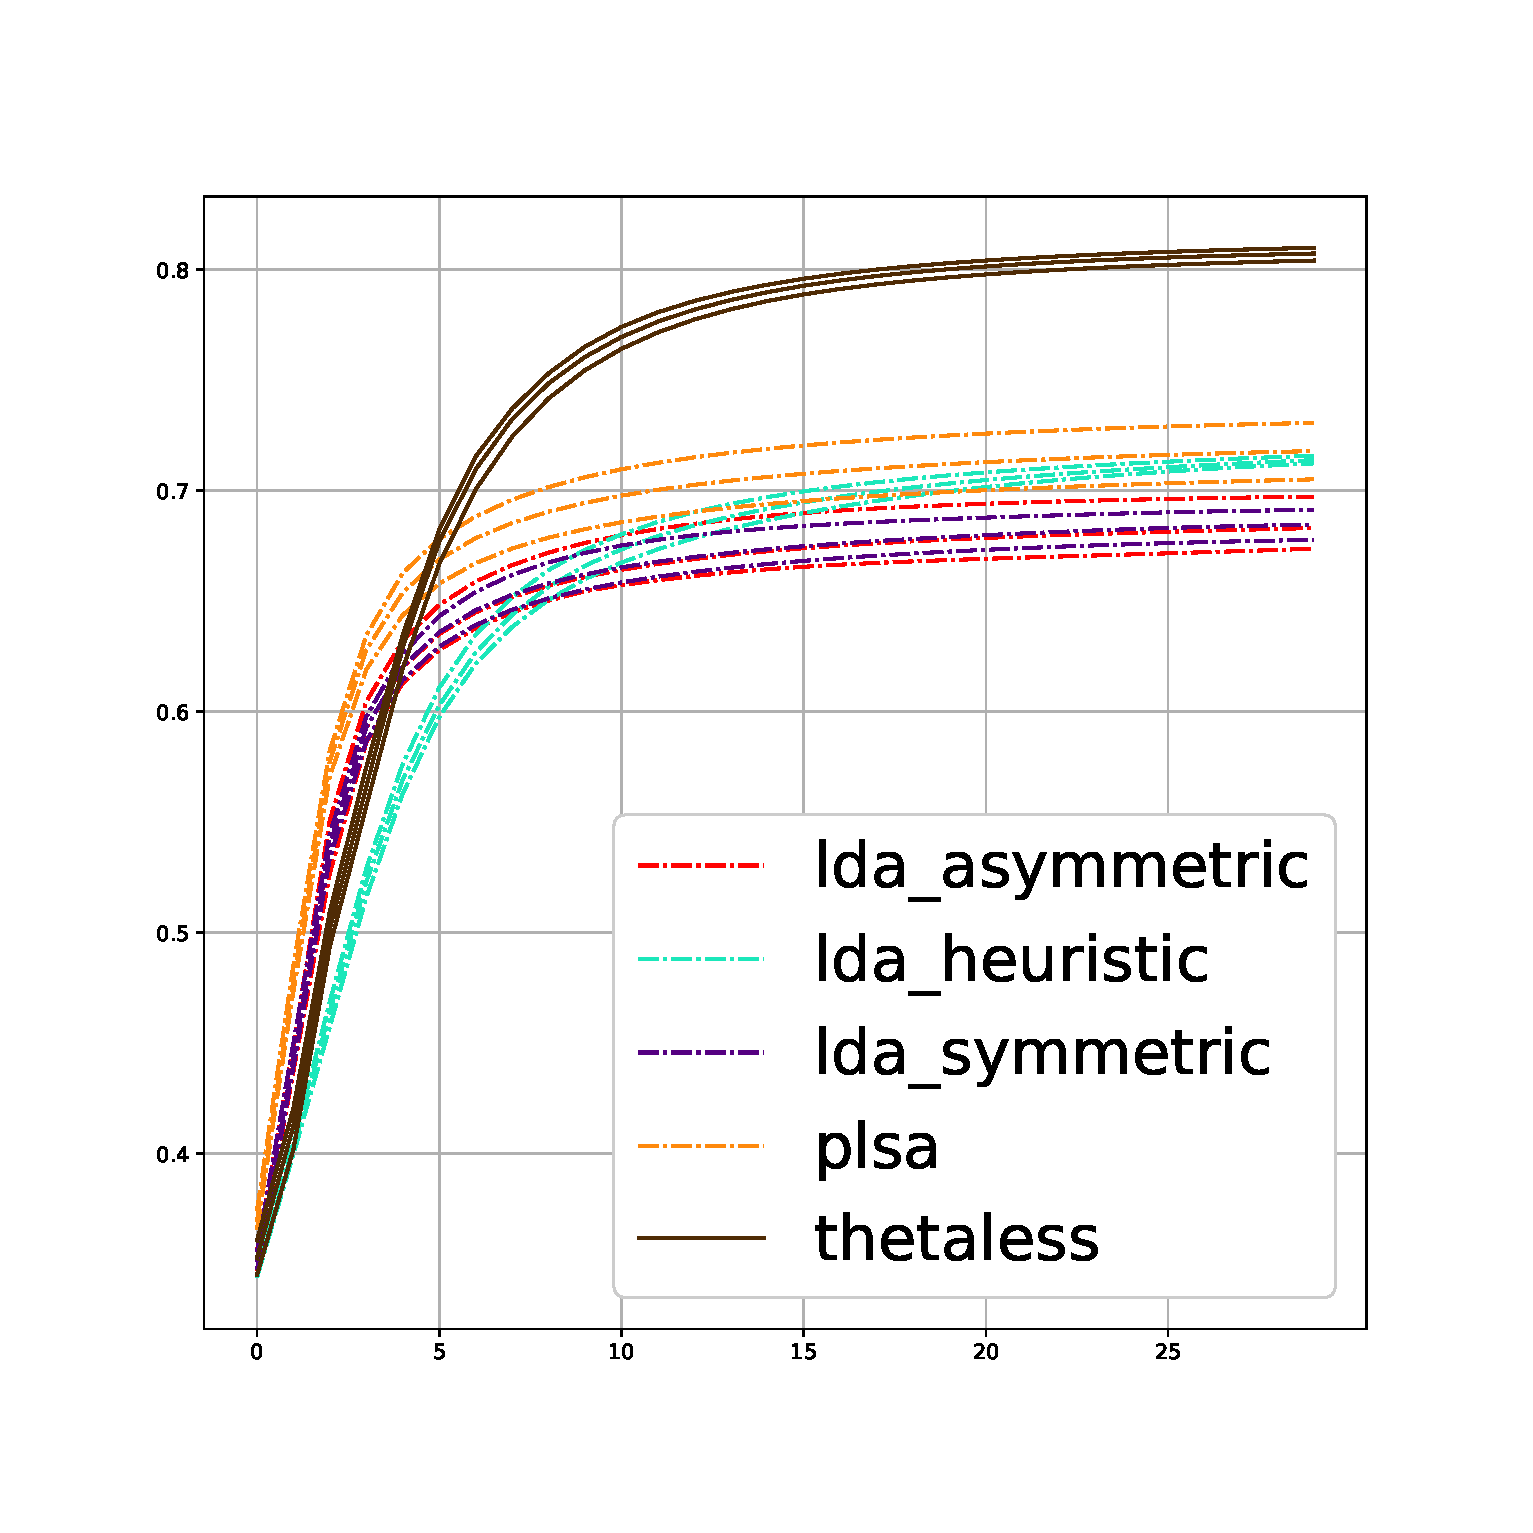
\includegraphics[width=54mm]{images/CH4_baselines_diversity_jensenshannon_False.eps}
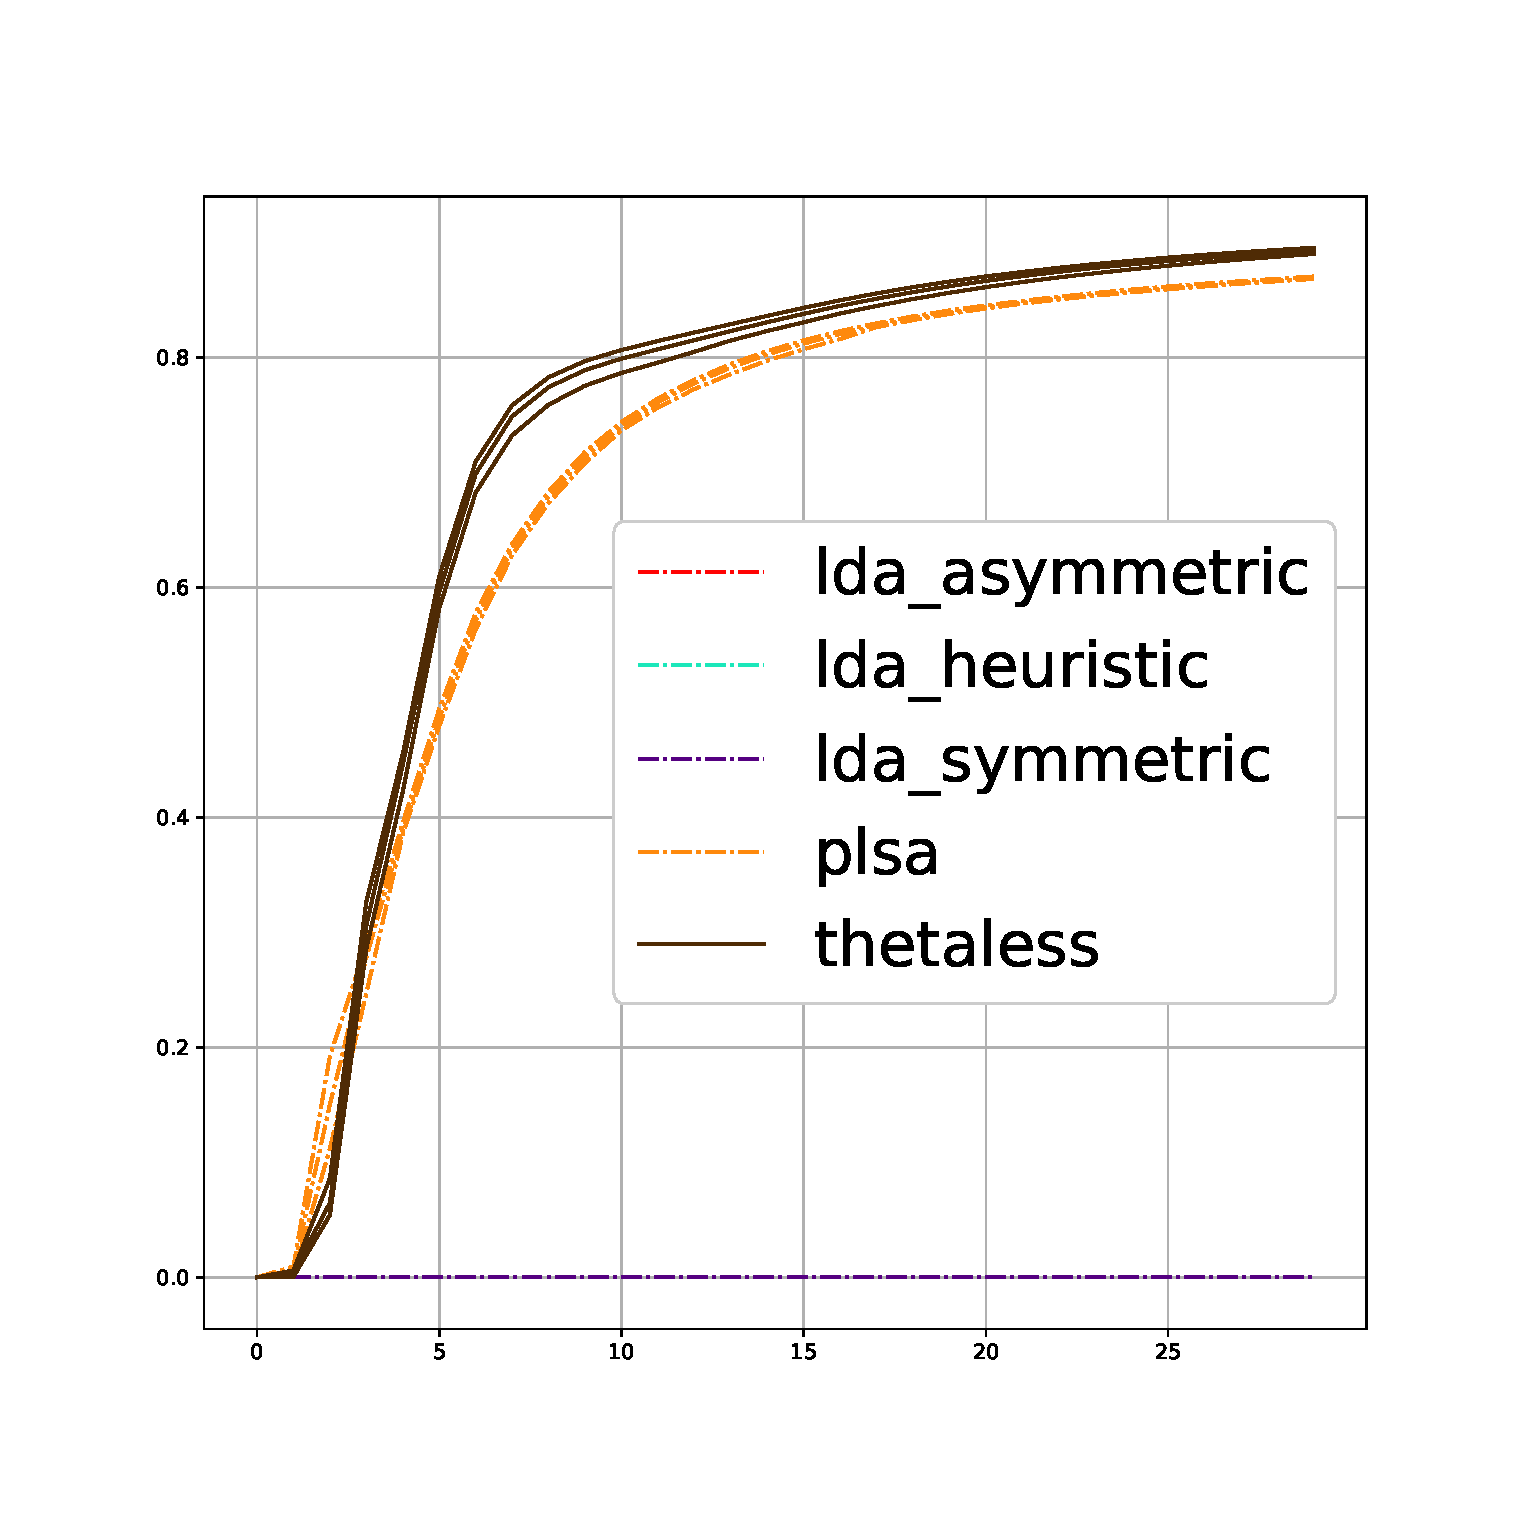
\includegraphics[width=54mm]{images/CH4_baselines_SparsityPhiScore.eps}& \end{tabular}
\end{figure}
Сравнение с базовыми моделями (PLSA и LDA с 3 видами приоров). Каждой модели соответствуют три линии: среднее значение, минимум и максимум (по пяти случайным перезапускам)
\end{frame}

\begin{frame}{Влияние на тематическую модель}

\begin{figure}
\setlength\tabcolsep{0pt} % default value: 6pt
\begin{tabular}{cc}
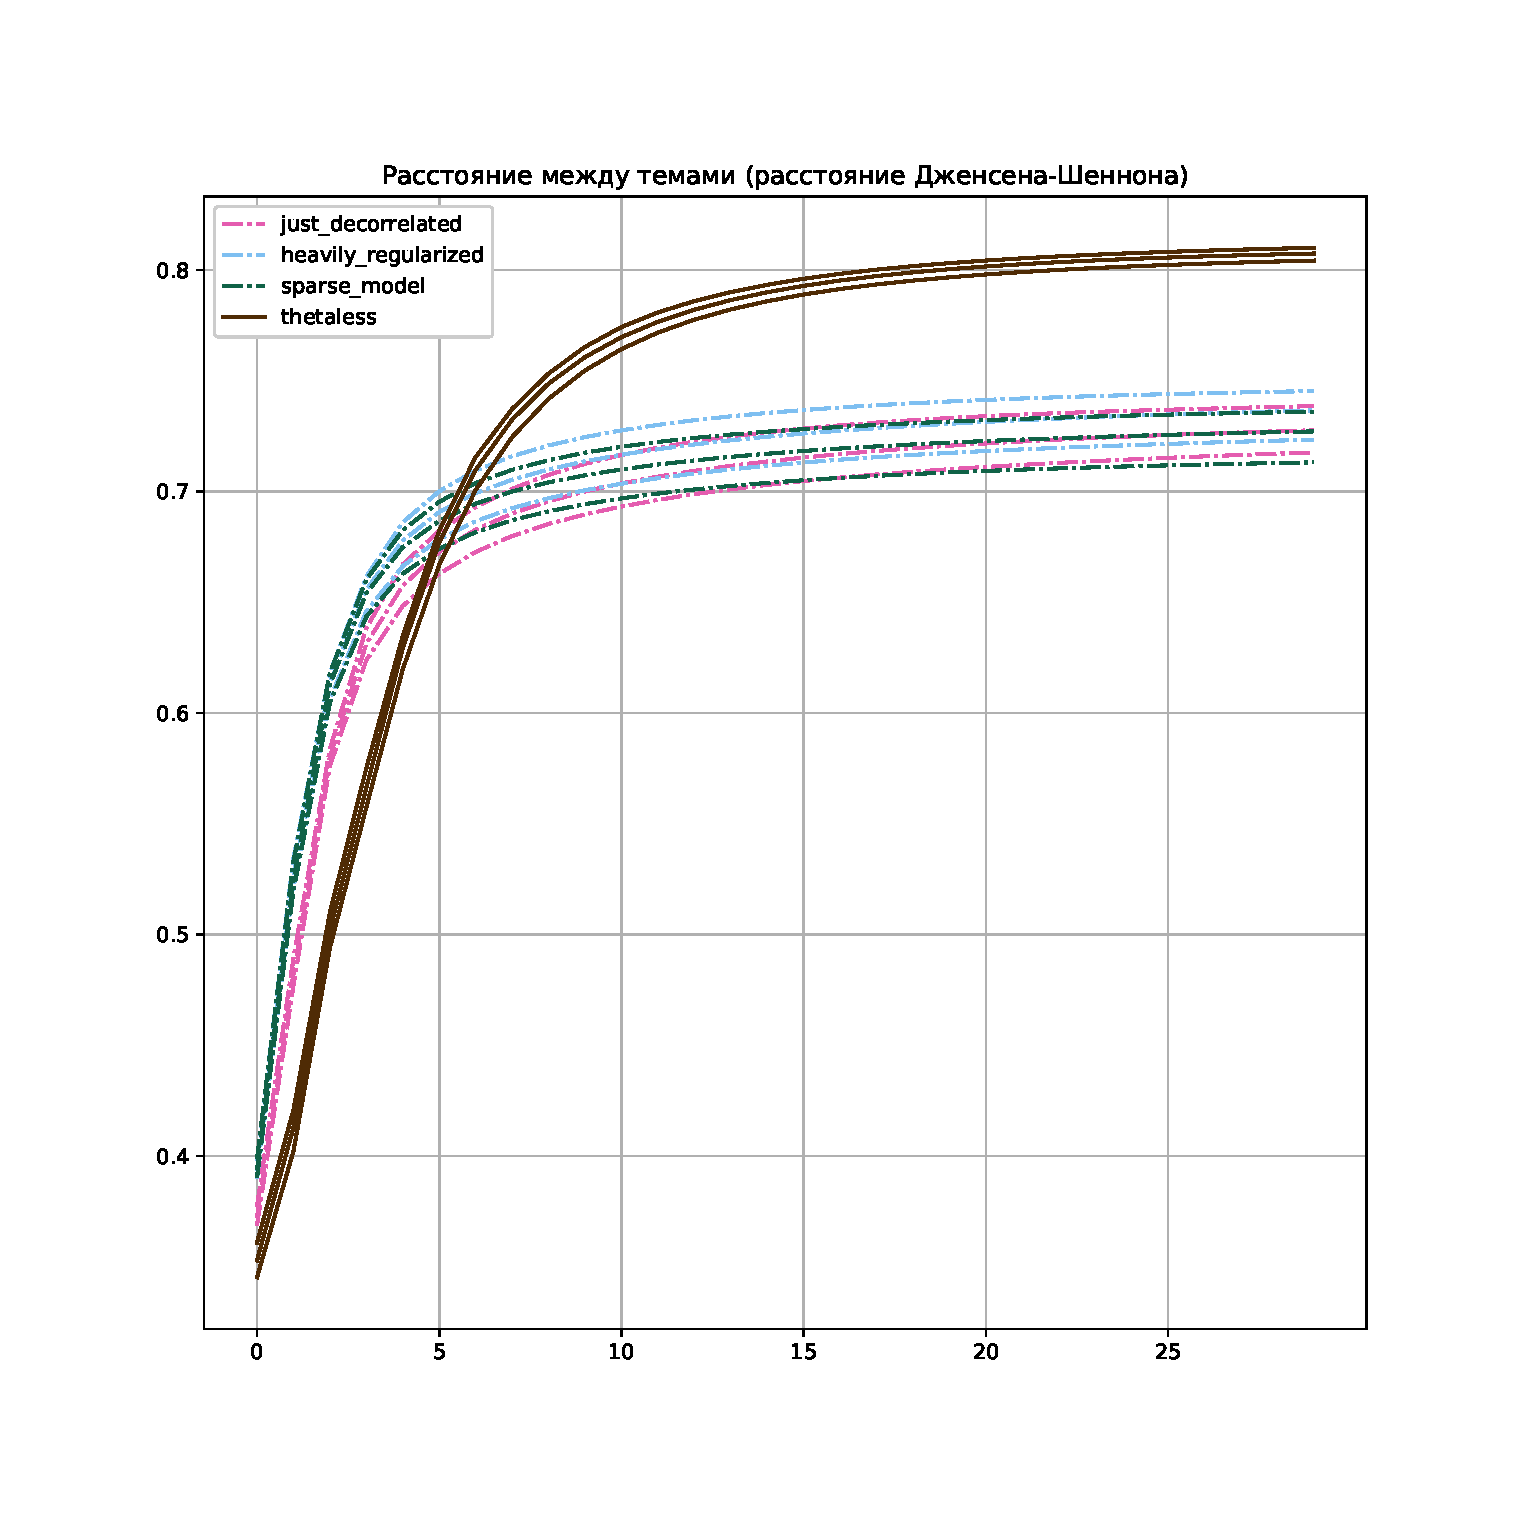
\includegraphics[width=54mm]{images/CH4_vs_regularized_diversity_jensenshannon_False.eps}
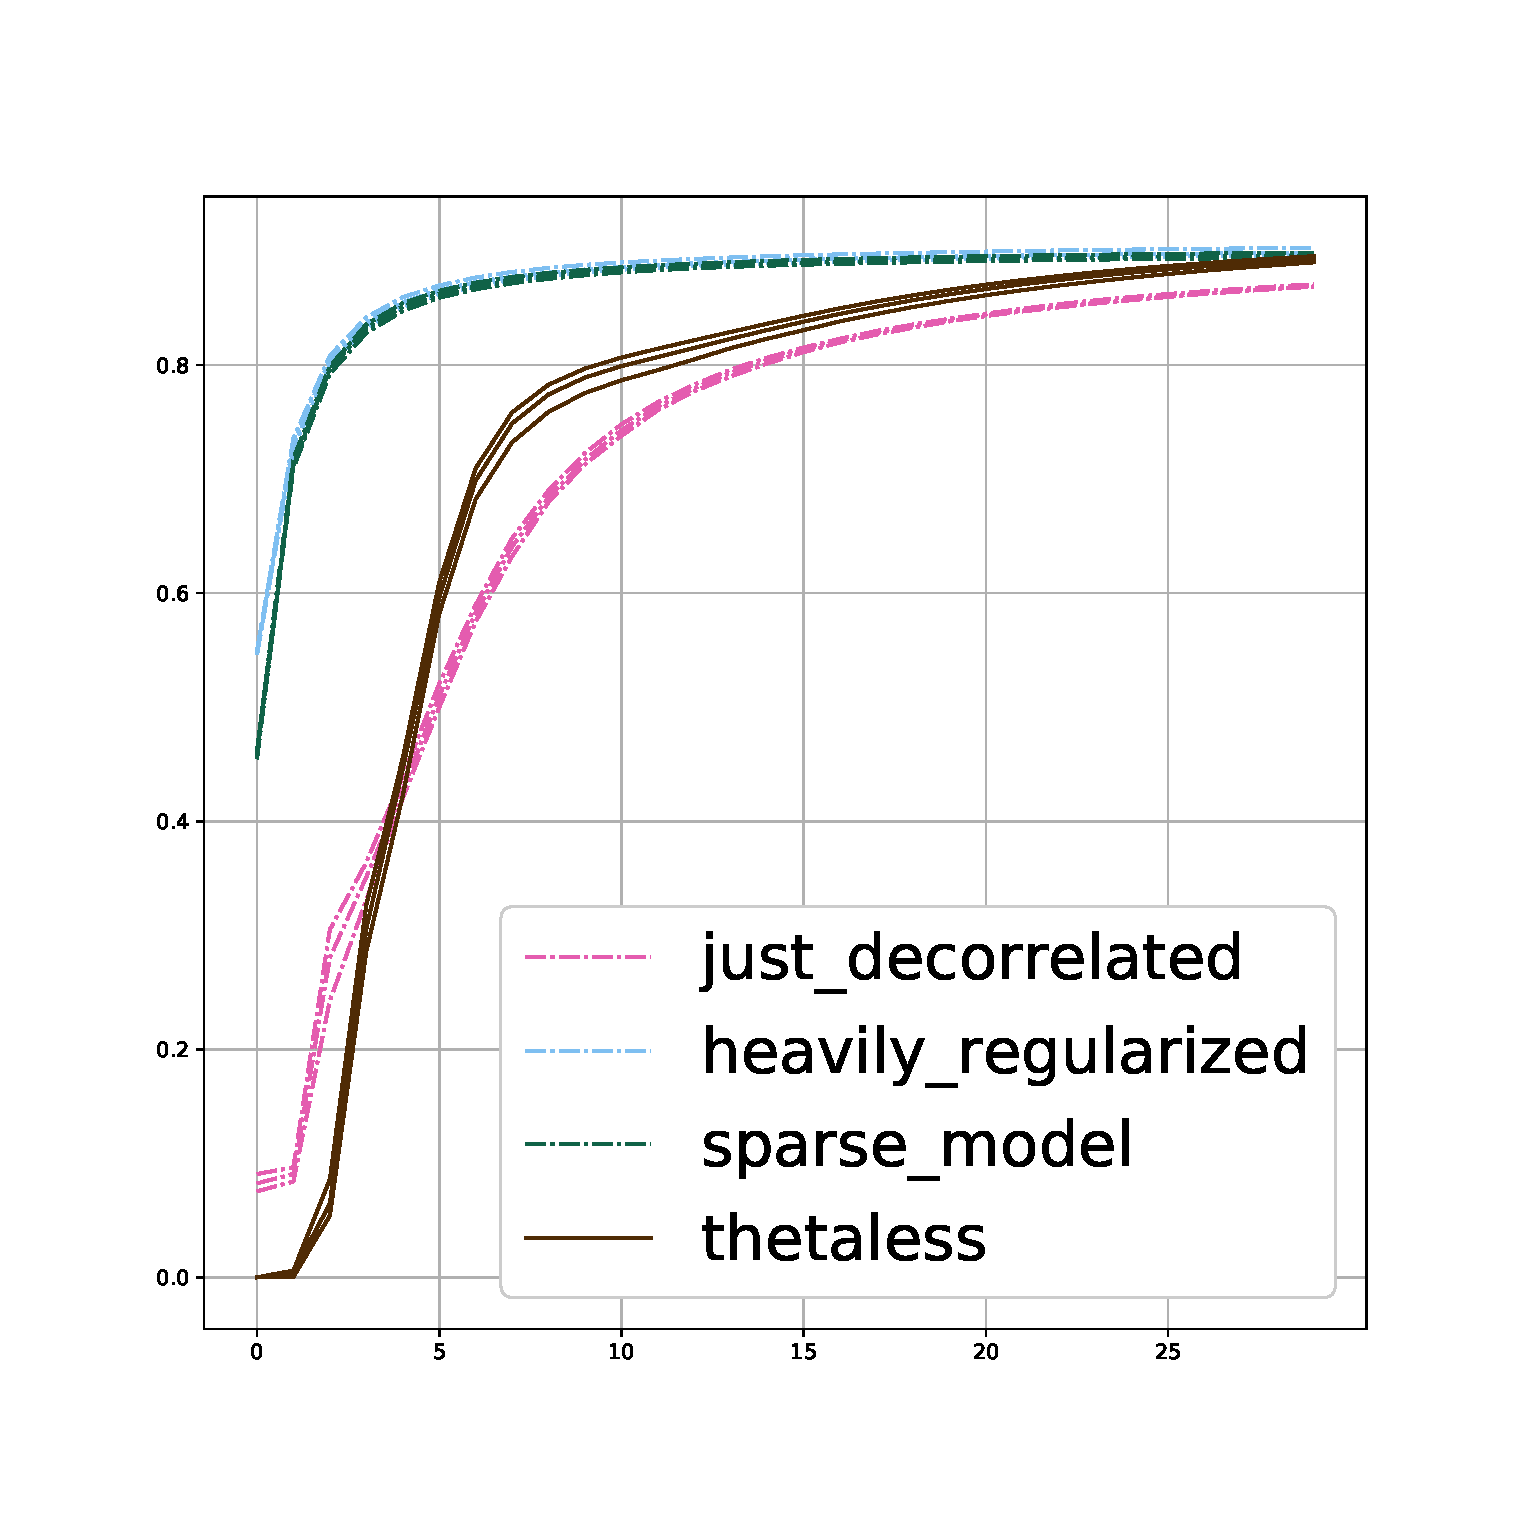
\includegraphics[width=54mm]{images/CH4_vs_regularized_SparsityPhiScore.eps}& \end{tabular}
\end{figure}
Сравнение с тремя аддитивно регуляризованными моделями
\end{frame}

\begin{frame}{Комбинирование с другими регуляризаторами}

\begin{figure}[t]
\setlength\tabcolsep{0pt} % default value: 6pt
\begin{tabular}{cc}
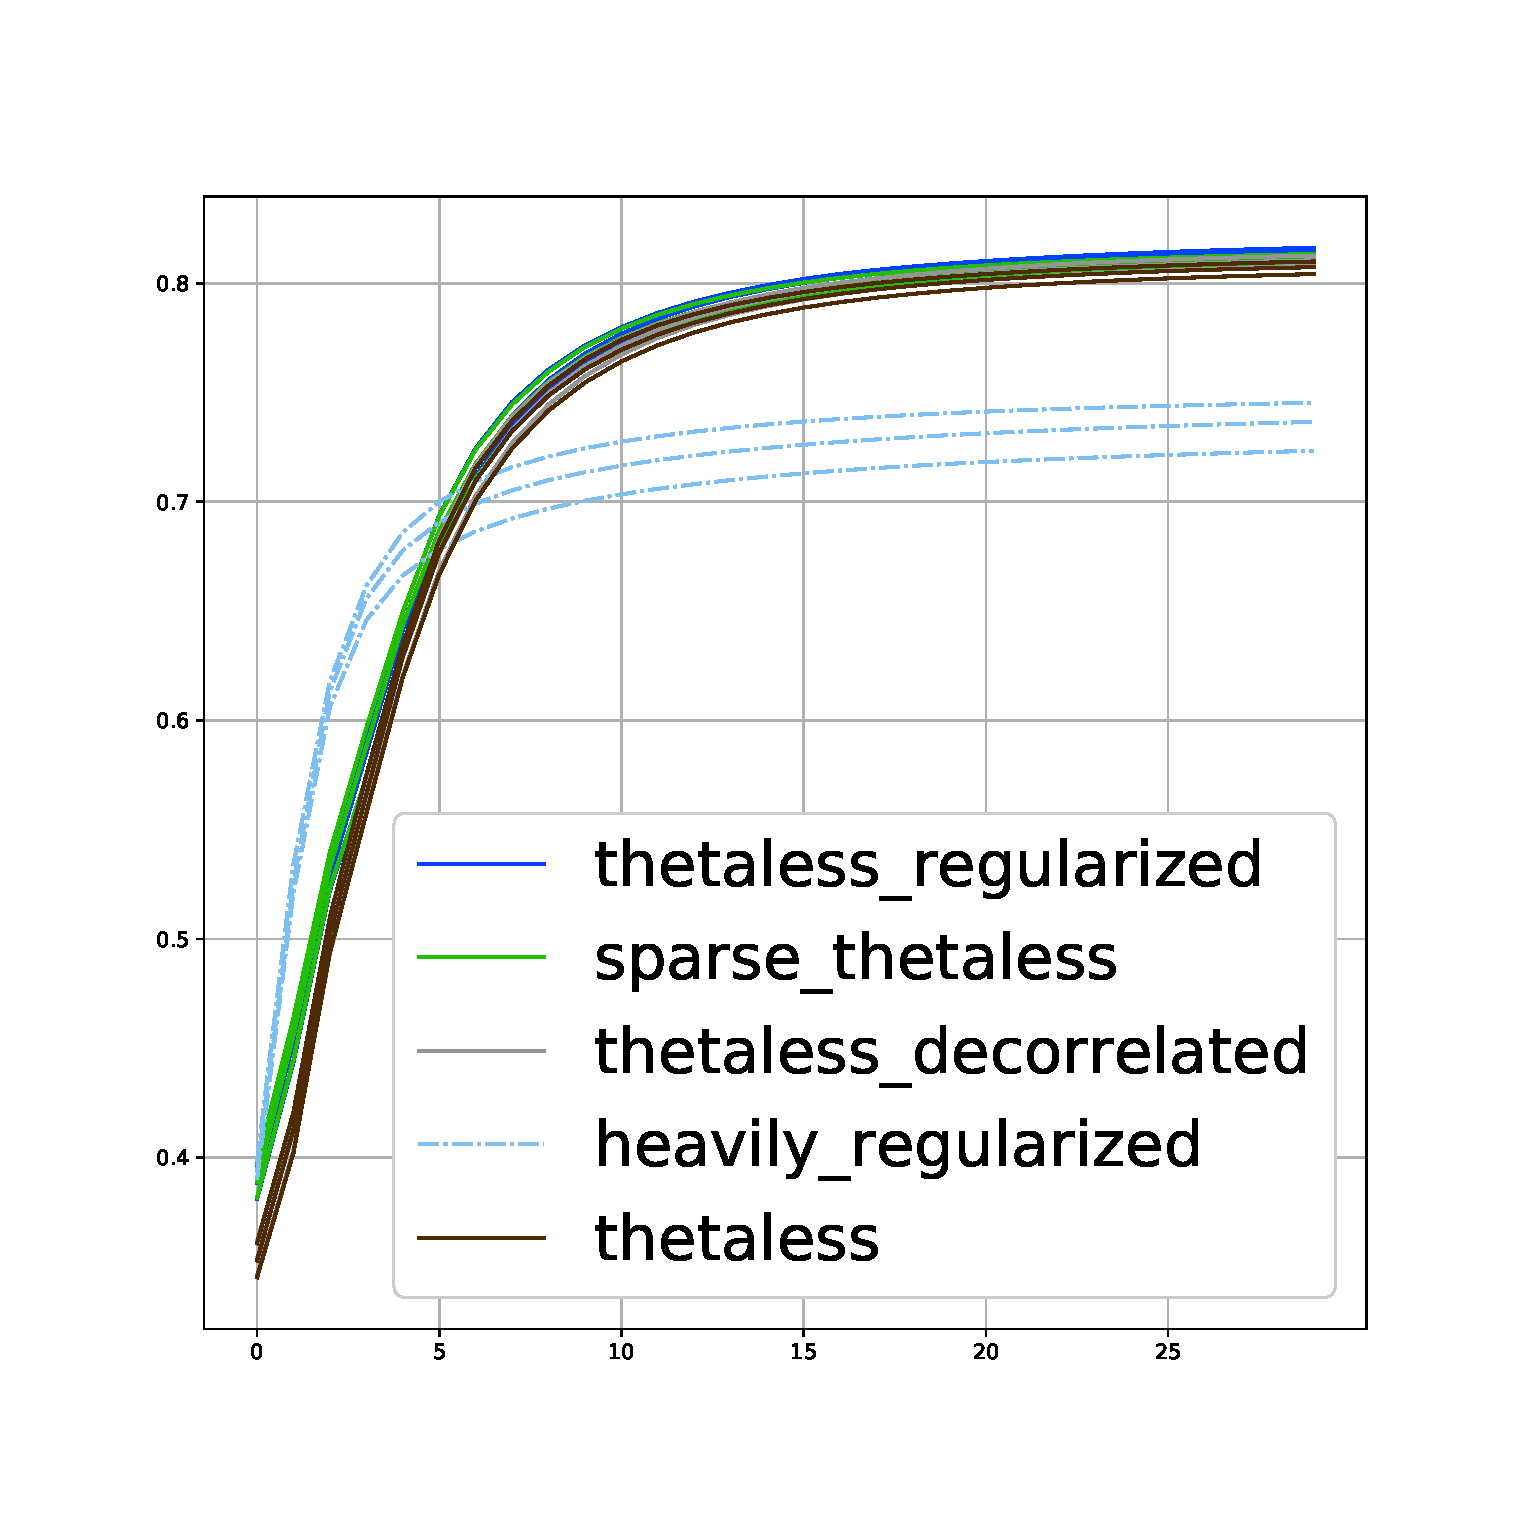
\includegraphics[width=54mm]{images/CH4_improved_diversity_jensenshannon_False.eps}
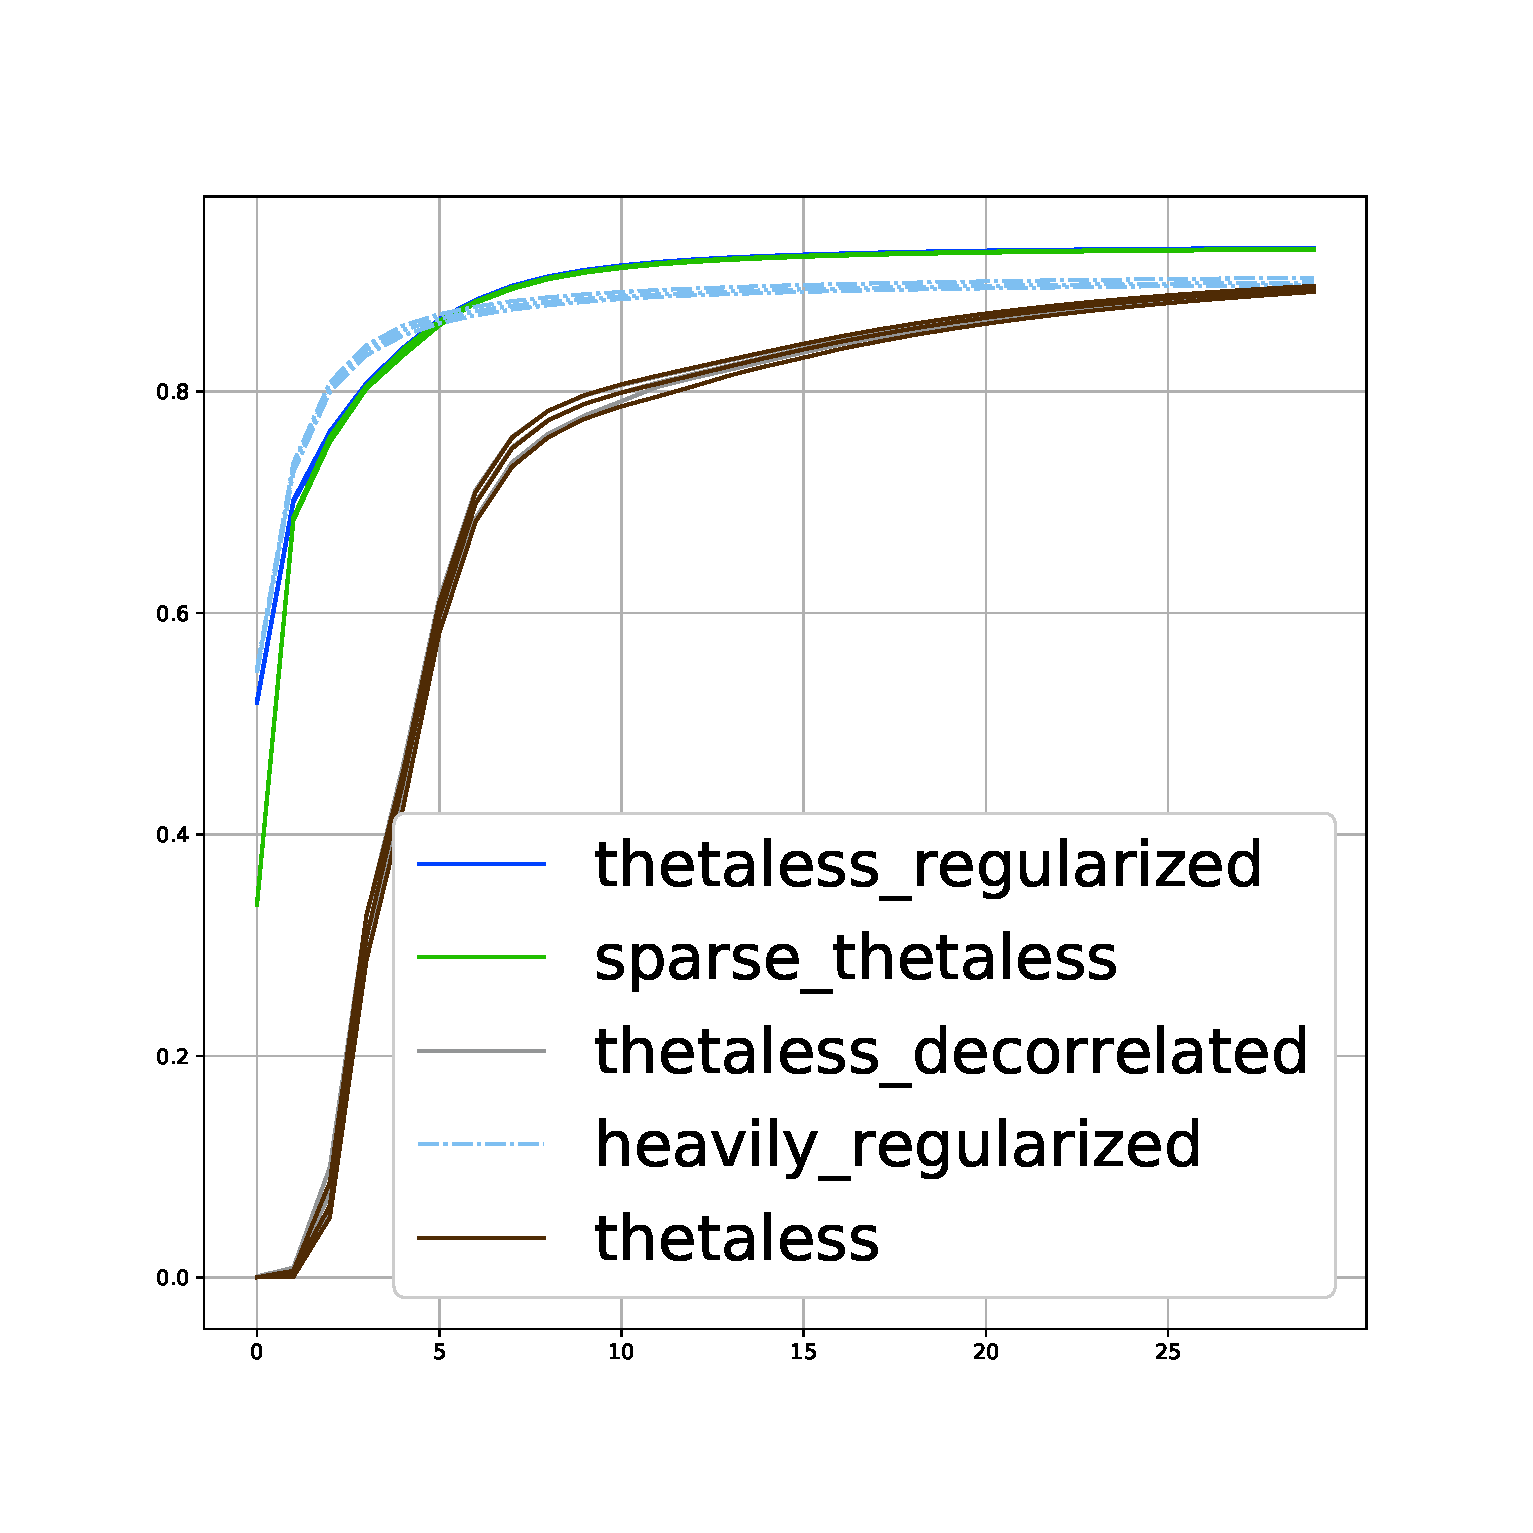
\includegraphics[width=54mm]{images/CH4_improved_SparsityPhiScore.eps}& \end{tabular}
\end{figure}
Псевдорегуляризатор успешно комбинируется с другими регуляризаторами ARTM, за счёт чего можно улучшить критерии качества ещё больше. 

Тематическая модель с псевдорегуляризатором и традиционным набором регуляризаторов (сглаживание фоновых тем, разреживание предметных тем, декорреляция) выигрывает у аналогичного ARTM по разреженности.

\end{frame}

\begin{frame}{Дерево эксперимента в библиотеке TopicNet}

\begin{figure}[ht]
    \centering
    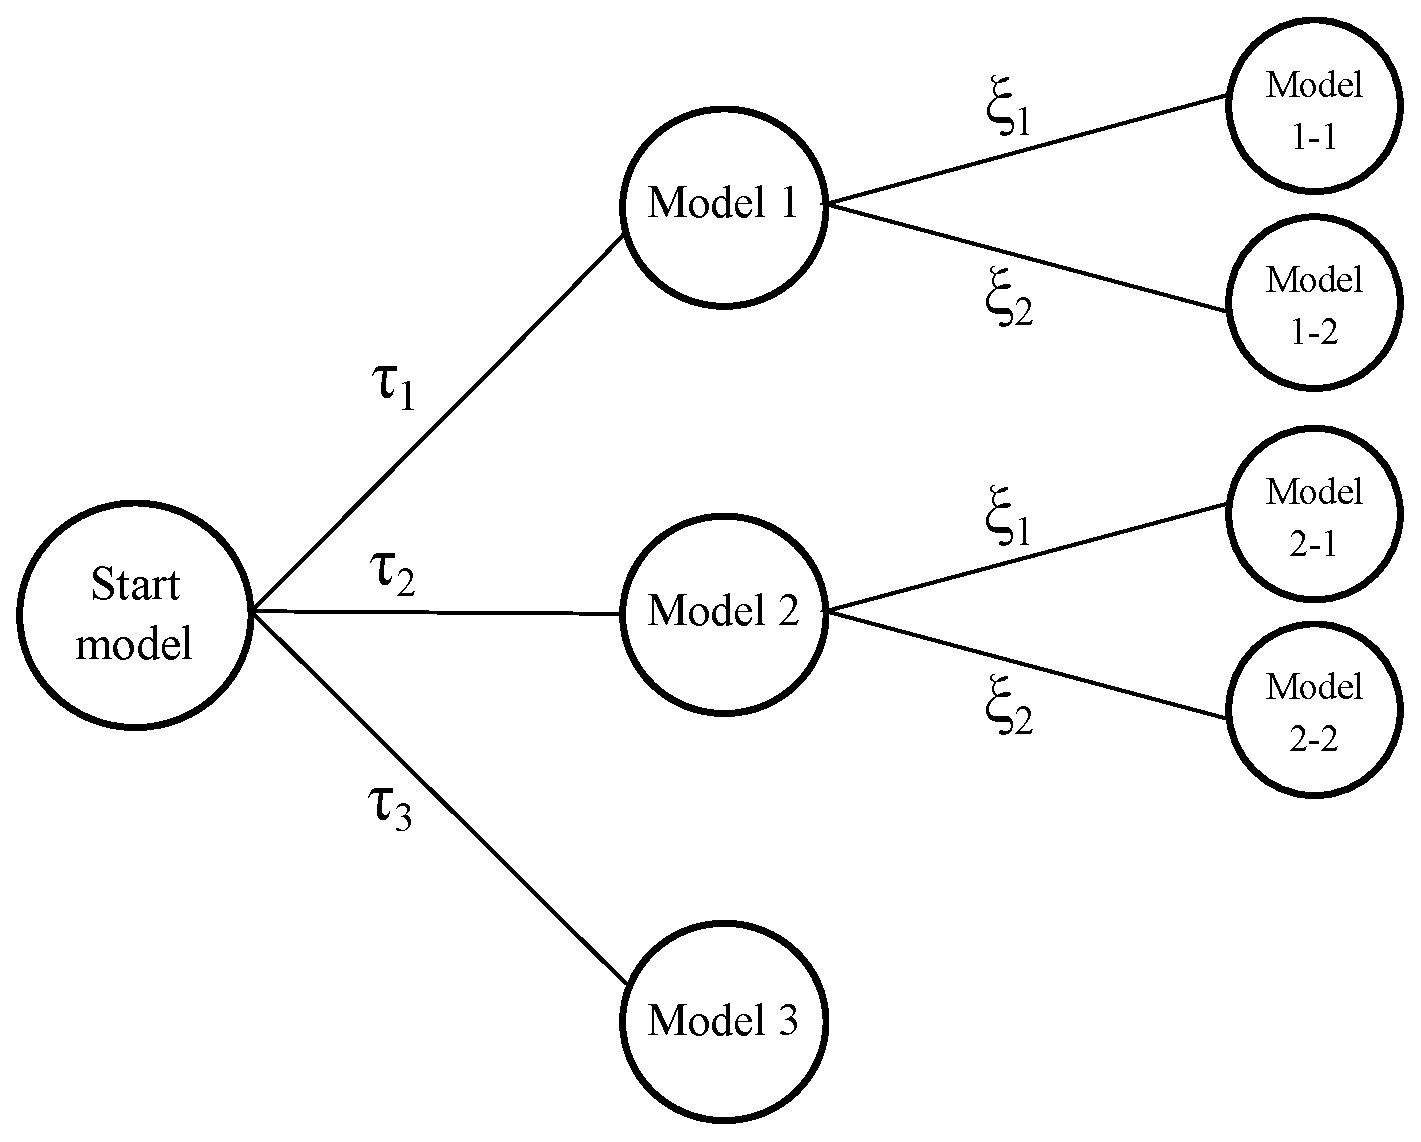
\includegraphics[width=0.6\textwidth]{training_scheme_example.eps}
\end{figure} 
        Первый этап: регуляризатор с $\tau \in \{\tau_1, \tau_2, \tau_3\}$.\\
        Лучшими оказываются \emph{Model 1} и \emph{Model 2}, они проходят на второй этап.\\
        К ним применяется другой регуляризатор с $\xi \in \{\xi_1, \xi_2\}$.
\end{frame}

\begin{frame}{Отбор моделей в библиотеке TopicNet}

Язык отбора моделей:

\begin{figure}[ht]
% \footnotesize
\raggedright
\texttt{TopicKernel@word.average\_contrast > 0.95 * MAXIMUM( \\
\hphantom{\ \ \ \ \ \ \ \ }TopicKernel@word.average\_contrast) \\
\hphantom{\ \ } and PerplexityScore@all < 1.1 * MINIMUM( \\
\hphantom{\ \ \ \ \ \ \ \ }PerplexityScore@all) \\
\hphantom{\ \ } and SparsityPhiScore@word -> max\\
\hphantom{\ \ } COLLECT 3} \\
\label{DSL-example}
\end{figure} 
	
%\begin{lstlisting}
%S -> <Expr> | <Expr> <Clct>
%<Clct> -> COLLECT <Int>
%<Expr> -> <Expr> AND <Expr>
%<Optr> -> less | eq | great
%<Expr> -> <Literal> <Optr> <Number>
%<Expr> -> <Literal> to MIN | <Literal> to MAX
%<Literal> -> <ScoreName> | model<ParameterName>
%\end{lstlisting} 

Поддержка пользовательским критериев качества:

\texttt{model.num\_topics == 10 and SparsityPhiScore\@word > MEDIAN(SparsityPhiScore\@word) and MyCustomScore -> max}

\end{frame}

\begin{frame}{Библиотека TopicNet}
	Тут будет про рецепты и конфиги в YAML-формате
\end{frame}

\begin{frame}{Конкуренты и <<параметры по умолчанию>>}


\end{frame}

\begin{frame}{TopicNet Thetaless vs GenSim}
Вспоминаем, что Thetaless повышает когерентность. Добавляем. Победили по всему.
\end{frame}


\begin{frame}{Таксономия обращений}
	Постановка задачи
\end{frame}

\begin{frame}{Таксономия обращений}
	Две разных коллекции. Примеры документов/тем из первой и из второй.
\end{frame}

\begin{frame}{Таксономия обращений}
    мы использовали пять модальностей
    среди них нграмы
	веса модальностей относительные: чиселки.
\end{frame}

\begin{frame}{Таксономия обращений}
	примеры тем модели

	можно гифку с иерархией тем?
\end{frame}

\begin{frame}[t]{Публикации и РИДы}
\footnotesize

Публикации в изданиях, индексируемых Scopus:
\begin{itemize}
    \smallskip\item  V. Alekseev, V. Bulatov, K. Vorontsov. Intra-text coherence as a measure of topic models’ interpretability  // Dialogue 2018

    \smallskip\item A. Popov, V. Bulatov, D. Polyudova, E. Veselova. Unsupervised dialogue intent detection via hierarchical topic model // RANLP 2019

    \smallskip\item V. Bulatov, V. Alekseev, K. Vorontsov, D. Polyudova, E. Veselova, A. Goncharov, E. Egorov. TopicNet: Making Additive Regularisation for Topic Modelling Accessible // LREC 2020

    \smallskip\item\color{red} И. А. Ирхин, В. Г. Булатов, К. В. Воронцов. Аддитивная регуляризация тематических моделей с быстрой векторизацией текста // Компьютерные исследования и моделирование, 2020
\end{itemize}

Зарегистрированные программы для ЭВМ в РФ:
\begin{itemize}
    \smallskip\item  Topic Net Cooking Machine  / Гончаров А. В., Булатов В. Г., Воронцов. К. В.; МФТИ. --- опубл. 17.09.2019, 2019662102

    \smallskip\item Система создания таксономии текстовой коллекции диалогового контактного центра / Гончаров А. В., Егоров. Е. О., Веселова. Е. Р., Булатов. В. Г.; МФТИ. --- опубл. 17.03.2020, 2020613851

    \smallskip\item Topic Net Viewers  / Гончаров А. В., Булатов В. Г., Воронцов. К. В.; МФТИ. --- опубл. 10.09.2019, 2019661840

\end{itemize}

\normalsize
\end{frame}


\begin{frame}
    \frametitle{Положения, выносимые на защиту}
\small
    \begin{itemize}
\item
    Методология построения тематических моделей, обеспечивающая формирование <<рецептов моделирования>> с автоматизированным подбором гиперпараметров по множеству критериев и отличающаяся использованием относительных коэффициентов регуляризации и кубов гиперпараметров.
\item
    Архитектура библиотеки TopicNet, обеспечивающая программную реализацию данной методологии и отличающаяся использованием удобного языка описания кубов гиперпараметров и возможностью создания пользовательских регуляризаторов и метрик качества на языке Python.
\item
    Универсальный рецепт моделирования, обеспечивающий многокритериальный выбор тематических моделей для широкого класса задач, отличающийся предварительной настройкой куба гиперпараметров по набору разнородных задач тематического моделирования.
\item
    Программная реализация нового критерия когерентности, обеспечивающая его эффективное вычисление и отличающаяся более полным использованием данных о сочетаемости слов внутри текстовых документов.
%\item
%    Программная реализация псевдорегуляризатора в библиотеке TopicNet, обеспечивающего быстрое однопроходное вычисление тематических векторных представлений документов и улучшение качества тематической модели по множеству критериев.
    \end{itemize}

    
\end{frame}
\note{
    Проговариваются вслух положения, выносимые на защиту
}
